\documentclass[11pt]{article}
\usepackage{amssymb}
\usepackage{graphicx}
\usepackage{float}
\usepackage{indentfirst}
\usepackage{subcaption}
\usepackage{booktabs}
\usepackage{setspace}
\usepackage{cite}
\usepackage[cmex10]{amsmath}
\interdisplaylinepenalty=2500 
\usepackage[usenames,dvipsnames]{xcolor}
\usepackage{pgfplots}
\usepackage{multirow}
\usepackage{hyperref}
\hypersetup{colorlinks,urlcolor=blue}
\usepackage{tikz}
\usepackage[americaninductors,americanresistors]{circuitikz}
\usepackage{listings}
\usetikzlibrary{shapes,arrows,positioning}
\usepackage{verbatim}
\usepackage[top=0.2in, bottom=1in, left=1in, right=1in]{geometry}
\usepackage{setspace}
\singlespacing
\graphicspath{{figures/}}
\pgfplotsset{width=7cm,compat=newest}

\def\width{12}
\def\height{4}

\definecolor{dkgreen}{rgb}{0,0.6,0}
\definecolor{gray}{rgb}{0.5,0.5,0.5}

\lstset{language=Matlab,
   keywords={break,case,catch,continue,else,elseif,end,equal,for,function,
      global,if,otherwise,persistent,return,switch,try,while},
   basicstyle=\ttfamily\footnotesize,
   keywordstyle=\color{blue},
   commentstyle=\color{dkgreen},
   stringstyle=\color{Plum},
   %numbers=left,
   numberstyle=\tiny\color{gray},
   stepnumber=1,
   numbersep=10pt,
   backgroundcolor=\color{white},
   tabsize=4,
   showspaces=false,
   showstringspaces=false,
   xleftmargin=-1in}

   \newcommand {\mtrx} [2] {
      $\left [ {
         \begin {array} {*{#1}c}
            #2
         \end {array}
         }  \right ]$
   }

\newcommand{\me}{\mathrm{e}}

\title{\textbf{Mobile Vital Radio} \\{\large ECE598HH Project Proposal} }

\author{Amr Khasaba, Brady Salz, Junheng Zhu}
\date{}
\begin{document}
\maketitle

For our project, we propose Mobile Vital Radio (\textbf{MoViRad}), a novel method of measuring physiological signals using a mobile device. We specifically focus on measuring the heartbeat and breathing rate of a person using frequency modulated continuous waves (FMCW). While past work exists that detects the breathing rate through use of a mobile device [Nandakumar et al. MOBISYS’15], they were ultimately unable to get down to the fine resolution required to measure heart beats. Our system precisely measures the phase by performing interpolation on individual bins in the FFT to get a theoretical accuracy of millimeters. 

% \begin{figure}[H]
% 	\centering
% 	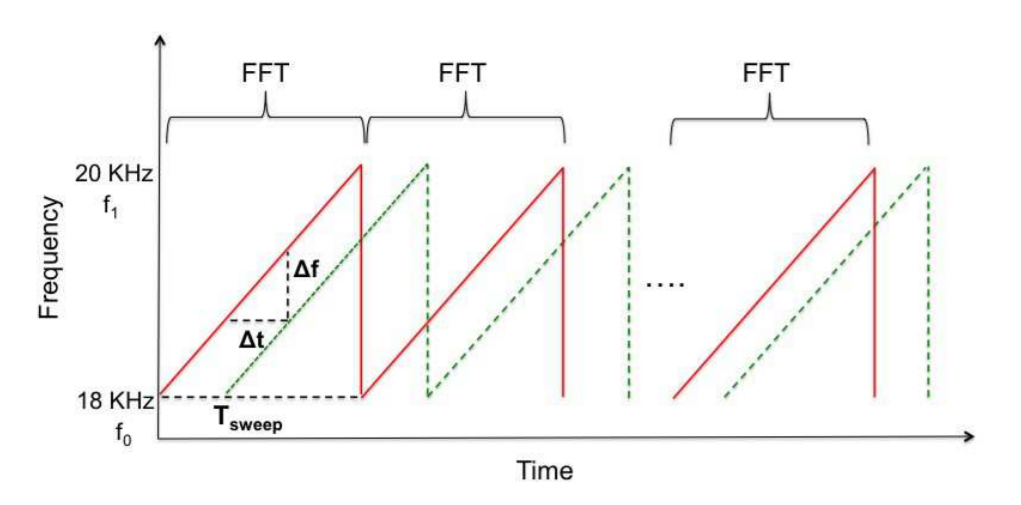
\includegraphics[scale=0.6]{fmcw.PNG}
% 	\caption{An Example FMCW transmission [Nandakumar et al. MOBISYS’15]}
% 	\label{fig:figure1}
% \end{figure}

In FMCW transmission, the frequency is linearly swept, resulting in a “chirp” signal being output. Our system uses a mobile phone’s speaker to broadcast this data as an acoustic wave. We measure the incoming reflection from the human body, and after downconverting by the broadcast frequency, we can find a coarse approximation of the delay via:
$$ \Delta f = \dfrac{f_{max} - f_{min}}{T_{\mathrm{sweep}}} \Delta t$$
where $\Delta t$ is the speed of the medium by the entire distance traveled. Since we use an acoustic wave, we'll approximate the speed of sound as a constant 340m/s. Using standard mobile phone specifications ($f_{s} = 44.1$kHz, $f_{\mathrm{speaker}} = 20$kHz), we get an coarse distance measurement of approximately 2cm. While adequate for breathing, this is not good enough to detect heartbeats. We then propose a novel fine tracking method for phase, in which we:
\begin{enumerate}
 	\item Perform a peak search in the correct bucket, assuming only one peak exist
 	\item Since the peak is very unlikely to fall exactly in one bin, we interpolate the peak and the second largest value to find a precise phase offset using the FFT
 	\item Use the previously mentioned coarse tracking plus the additional fine tracking to get precise distance measurements
\end{enumerate} 
Our interpolation method revolves around the definition of the FFT. By taking the ratio of two consecutive samples (the peak $k$, and next highest point $k+1$), we wil find a ratio $R$:
$$ R = \dfrac{X[k]}{X[k+1]} = \dfrac{1 - r e^{-\frac{j2\pi}{N}}}{1 -r}$$
where $r$ is the frequency shift $e^{\frac{j2\pi\delta}{N}}$ and $\delta$ is our fine frequency offset. We can solve for $r$ now as a function of $R$, and extract the phase information from that.

This fine estimate is as accurate as our spectrum is. When we have multiple close peaks such that our coarse FFT can not resolve them individually, we will have large errors. However, assuming we can isolate each frequency such that there are distinct peaks between them, we can achieve much higher levels of accuracy. Assuming we sweep from 10kHz to 20kHz, with a 1m maximum distance and a sweep time of 50ms, with only one signal we can find achieve a maximum distance error of 0.25mm. In prescence of three signals, each 5cm apart distance, we still maintain a maximum error of 7.2mm.
\end{document}